\chapter{Теоретический раздел}

AES (in English, Advanced Encryption Standard)~---~симметричный алгоритм блочного шифрования (размер блока 128 бит, ключ 128/192/256 бит), принятый в качестве стандарта шифрования правительством США по результатам конкурса AES. Этот алгоритм хорошо проанализирован и сейчас широко используется, как это было с его предшественником DES. Национальный институт стандартов и технологий США опубликовал спецификацию AES 26 ноября 2001 года после пятилетнего периода, в ходе которого были созданы и оценены 15 кандидатур. 26 мая 2002 года AES был объявлен стандартом шифрования.

Для AES рекомендовано несколько режимов:

\begin{itemize}
	\item ECB (electronic code book)~---~режим «электронной кодовой книги» (простая замена);
	\item CBC (cipher block chaining)~---~режим сцепления блоков;
	\item PCBC (propagating cipher block chaining)~---~режим распространяющегося сцепления блоков;
	\item CFB (cipher feed back)~---~режим обратной связи по шифротексту;
	\item OFB (output feed back)~---~режим обратной связи по выходу;
	\item Counter Mode (CM)~---~режим счётчика.
\end{itemize}

\section{Алгоритм AES}

Псевдокод алгоритма AES.

\begin{lstlisting}[language=Pascal, label=lst:pseudoaes, caption={Псевдокод алгоритма AES}]
Cipher(byte in[4*Nb], byte out[4*Nb], word w[Nb*(Nr+1)])
begin
    byte state[4,Nb]
    
    state = in

    AddRoundKey(state, w[0, Nb-1])

    for round = 1 step 1 to Nr-1
        SubBytes(state)
        ShiftRows(state)
        MixColumns(state)
        AddRoundKey(state, w[round*Nb, (round+1)*Nb-1])
    end for

    SubBytes(state)
    ShiftRows(state)
    AddRoundKey(state, w[Nr*Nb, (Nr+1)*Nb-1])

    out = state
end
\end{lstlisting}


Расшифрование представляет собой тот же алгоритм, запущенный в обратном порядке.

\newpage

\section{Алгоритм OFB}

На рисунках \ref{fig:ofb_enc.jpeg}--\ref{fig:ofb_dec.jpeg} изображены схемы шифрования и расшифрования с использованием алгоритма OFB.

\begin{figure}[h!]
\centering
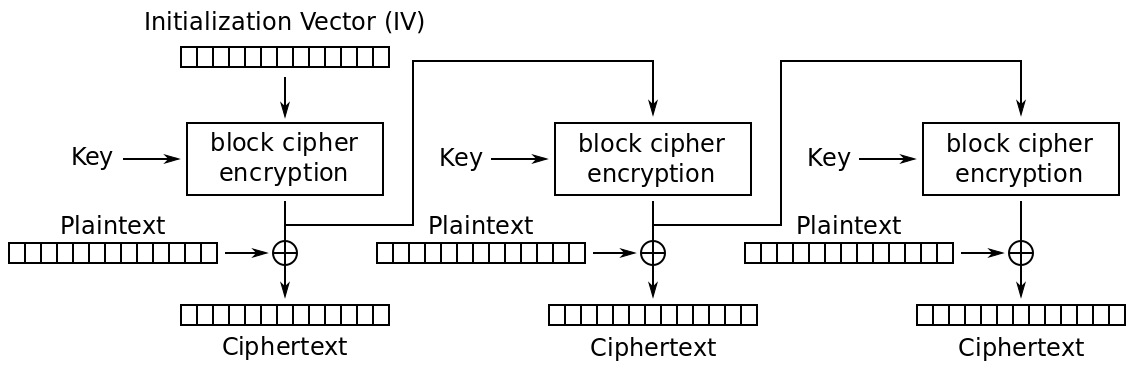
\includegraphics[width=0.75\textwidth]{assets/ofb_enc.jpeg}
\caption{Шифрование с использованием OFB}
\label{fig:ofb_enc.jpeg}
\end{figure}

\begin{figure}[h!]
\centering
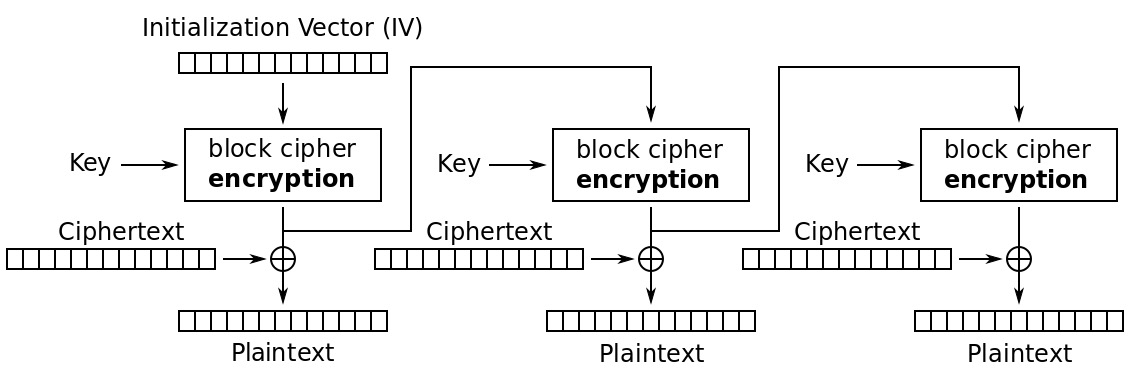
\includegraphics[width=0.75\textwidth]{assets/ofb_dec.jpeg}
\caption{Расшифрование с использованием OFB}
\label{fig:ofb_dec.jpeg}
\end{figure}


